\chapter{アイソジオメトリック解析手法}

\section{非一様有理Bスプライン(Non-Uniform Rational B-Spline, NURBS)}
非一様有理Bスプライン(Non-Uniform Rational B-Spline, NURBS)は,エンジニアリングデザインの中で最も広く使用される幾何学表現である.
コントロールポイントと重みを適切に設定することで,円弧等の曲線や曲面を厳密に表現できるという特徴があり,CADの形状表現にも用いられている.
NURBSはBスプライン(B-Spline)に重みを導入することで構成されており,Bスプラインは,コントロールポイントとノットベクトル,次数によって構成される.

\subsection{ノットベクトル}
Bスプラインのパラメータ空間は,パッチと呼ばれる範囲内での小領域に対してローカルに定義されるものであり,図~\ref{fig:parameter space}のように
パラメータ空間は物理空間の写像となっている.

\begin{figure}[htbp]
  \centering
  \includegraphics[keepaspectratio, scale = 1.2]
  {fig/物理空間とパラメータ空間.ai}
  \caption{B-Spline Physical space and Parametric space}
  \label{fig:parameter space}
\end{figure}

ノットベクトル(Knot vector)とは,区分的に構成されるBスプラインをつなぐ役割を持つパラメータ空間座標の座標の並びを示す単調増加のベクトルであり,パラメータ空間の
座標値$\xi, \eta$を用いて$\boldsymbol{\Xi} = \{\xi_0, \xi_1, \xi_2, \dots, \xi_{n+p}\}, \boldsymbol{H} = \{\eta_0, \eta_1, \eta_2, \dots, \eta_{m+q}\}$
と書かれる.ここで,$n, m$はBスプラインを構成するコントロールポイントの数,$p,q$は基底関数の次数である.
コントロールポイント(Control point)は物理空間上の座標であり,各軸方向のコントロールポイント数がパラメータ空間での各軸方向の基底関数の個数となる.
ノットベクトルは$n + p + 1$個の成分(ノット)によって構成される.

パラメータ空間で複数のノットを同じ値にすると,これらは重複ノットと呼ばれ,そのノットの数を重複度と呼ぶ.
IGA解析では一般に一様オープンノットベクトルと呼ばれる,最小と最大の値のノットを$p + 1$回重複させ,
他のノットを等間隔に設定したノットベクトルを用いる.
これによってBスプライン曲線の端点を表現でき,パラメータ空間上で要素を等分割することができる.
また,パラメータ空間は,物理空間の写像であるため,$\xi, \eta$の範囲は自由に設定することができるが,
プログラムの関係上,0から1までに設定するのが一般的である.

\subsection{Bスプライン基底関数}
Bスプライン基底関数はノット$\xi$を用いて以下のように表される.$p = 0$のとき

\begin{equation}
  N_{i,0}(\xi)= \left \{
  \begin{array}{l}
    1    \ \qquad $if$\  \xi_{i} \leq \xi < \xi_{i + 1} \\
    0    \ \qquad $otherwise$
  \end{array}
  \right.
  \label{eq:basis func 0}
\end{equation}

\noindent
$p = 1,2,3,\dots$のとき

\begin{equation}
  N_{i,p}(\xi)=
  \frac{\xi-\xi_i}{\xi_{i+p}-\xi_i}N_{i,p-1}(\xi)
  +\frac{\xi_{i+p+1}-\xi}{\xi_{i+p+1}-\xi_{i+1}}N_{i+1,p-1}(\xi)
  \label{eq:basis func 1}
\end{equation}

\noindent
ここで,$N_{i,p}$は次数$p$の$i$番目のBスプライン基底関数を表している.
Bスプライン基底関数には以下のような性質がある.

\begin{enumerate}
  \item 単位分割(Partition of Unity)の性質を有する.$\forall \xi$,
    \begin{equation}
      \sum_{i = 0}^{n - 1} N_{i, p}(\xi) = 1
    \end{equation}
  \item それぞれの基底関数は負の値にならない.$\forall \xi$,
    \begin{equation}
      N_{i,p}(\xi) \geq 0
    \end{equation}
  \item それぞれの$p$次の基底関数は要素境界(ノット境界)をまたいで$C^{p-1}$の連続性を持つ.
  \item ノットの重複度が$k$であるとき,そのノット上で基底関数は$C^{p-k}$連続となる.
  \item 次数$p$のBスプライン基底関数のサポートは常に$p+1$のノット間隔で行われる.
\end{enumerate}

例として,一様オープンノットベクトル$\boldsymbol{\Xi}=\{0,0,0,0.25,0.5,0.75,1,1,1, 1, 1\}$に対する
2次のBスプライン基底関数の分布を図~\ref{fig:basis func}に示す.

\begin{figure}[htbp]
  \centering
  \includegraphics[keepaspectratio, scale = 1.1]
  {fig/basis_func.ai}
  \caption{B-Spline basis function}
  \label{fig:basis func}
\end{figure}

\newpage

また,Bスプライン基底関数の導関数はノットベクトルと基底関数の次数を用いて以下のように表される.

\begin{equation}
  \label{eq:d of B-spline shape func}
  \frac{d}{d\xi}N_{i,p}(\xi) = \frac{p}{\xi_{i+p} - \xi_i}N_{i,p-1}(\xi) - \frac{p}{\xi_{i+p+1} - \xi_{i+1}}N_{i+1,p-1}(\xi)
\end{equation}

\subsection{Bスプライン曲線}
Bスプライン曲線は物理空間上の座標であるコントロールポイントを用いて線形結合で表される.
$n$個のコントロールポイント$\boldsymbol{B}_i(i = 0, 1, \dots, n-1)$,Bスプライン基底関数$N_{i, p}(i = 0, 1, \dots, n-1)$,
次数$p$,ノットベクトル$\boldsymbol{\Xi} = \{\xi_0, \xi_1, \dots, \xi_{n+p}\}$とすると,
Bスプライン曲線$\boldsymbol{C}(\xi)$は以下のように表される.

\begin{equation}
  \boldsymbol{C}(\xi)=\sum_{i=0}^{n-1} N_{i,p}(\xi)\boldsymbol{B}_i
\end{equation}

例として,一様オープンノットベクトル$\boldsymbol{\Xi}=\{0,0,0,0.25,0.5,0.75,1,1,1\}$,
コントロールポイント$\boldsymbol{B} = \{(1,2),(2,1),(3,1),(3,3),(5,3),(2,5)\}^T$に対する
2次のBスプライン曲線を図~\ref{fig:b-spline curve}に示す.

\begin{figure}[htbp]
  \centering
  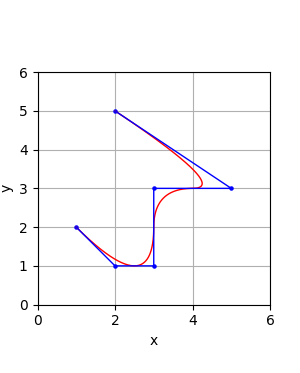
\includegraphics[keepaspectratio, scale = 1.0]
  {fig/png/03.png}
  \caption{B-Spline curve and control points}
  \label{fig:b-spline curve}
\end{figure}

\newpage

\subsection{NURBS基底関数・NURBS曲線}
NURBS基底関数はBスプライン基底関数に重み(Weight)を導入した関数であり,有理式(分数式)で表現される.
NURBS曲線は,形状を制御するための要素として各コントロールポイントに対してスカラーの重みを設定し,
Bスプライン曲線を中心投影によって通常座標空間上に射影することで得られる.
$n$個のコントロールポイント$\boldsymbol{B}_i(i = 0, 1, \dots, n-1)$,重み$w_i(i = 0, 1, \dots, n-1)$,次数$p$,
Bスプライン基底関数$N_{i,p}$とすると,NURBS基底関数$R^p_i(\xi)$とNURBS曲線$\boldsymbol{C}(\xi)$は以下のように表される.

\begin{align}
  \label{eq:weight func}
  W(\xi) &= \sum_{\hat{i}=0}^{n-1}N_{\hat{i},p}(\xi)w_{\hat{i}}\\
  R^{p}_{i}(\xi)&=\frac{N_{i,p}(\xi)w_i}{W(\xi)}=\frac{N_{i,p}(\xi)w_i}{\sum_{\hat{i}=0}^{n-1}N_{\hat{i},p}(\xi)w_{\hat{i}}}\\
  \boldsymbol{C}(\xi)&=\sum_{i=0}^{n-1}R^{p}_{i}(\xi)\boldsymbol{B}_i
\end{align}

また,基底関数の次数$p$とすると
NURBS基底関数の導関数は式~(\ref{eq:d of B-spline shape func})と式~(\ref{eq:weight func})を用いて以下のように表される.

\begin{align}
  \label{eq:d of NURBS shape func}
  \frac{d}{d\xi} R^p_i (\xi) &= w_i \frac{W(\xi)N_{i,p}' - W'(\xi)N_{i,p}(\xi)}{(W(\xi))^2} \\
  W'(\xi) &= \sum^{n - 1}_{\hat{i} = 0} N'_{\hat{i},p}(\xi)w_{\hat{i}}\\
  N'_{i,p}(\xi) &\equiv \frac{d}{d\xi}N_{i,p}
\end{align}


重みは基底関数が2次の場合,図~\ref{fig:weight}に示すようなコントロールポイント
$\boldsymbol{B_1},\boldsymbol{B_2},\boldsymbol{B_3}$と重み$w_1,w_2,w_3$,
角度$\theta$を考えると,以下のように設定することで円弧を表現できる.

\begin{align}
  w_1 &= w_3 = 1\\
  w_2 &= \cos{\frac{\theta}{2}}
\end{align}

\begin{figure}[htbp]
  \centering
  \includegraphics[keepaspectratio, scale = 1.7]
  {fig/weight.ai}
  \caption{How to set weights in NURBS}
  \label{fig:weight}
\end{figure}

\newpage

Bスプライン曲線とNURBS曲線を比較した図を図~\ref{fig:compare nurbs}に示す.
コントロールポイント数や次数に依らず,適切に重みを設定したNURBS曲線は円弧と厳密に一致する.

\begin{figure}[htbp]
  \centering
  \includegraphics[keepaspectratio, scale = 0.9]
  {fig/compare_nurbs.ai}
  \caption{A comparison of B-Spline curve and NURBS curve}
  \label{fig:compare nurbs}
\end{figure}

\noindent
このNURBS基底関数を用いることにより,円錐曲線や二次曲線の正確な描写が可能となり,
重みを制御することで幾何形状の微調節も可能となる.

\subsection{NURBS曲面}
NURBS曲面は$\xi$方向の次数$p$,$\eta$方向の次数$q$,
コントロールネット$\boldsymbol{B}_{i,j}$,
重み$w_{i,j} (i=0, 1, \dots, n-1,  j=0,1, \dots, m-1)$とすると,
NURBS基底関数$R^{p,q}_{i,j}(\xi, \eta)$とNURBS曲面$\boldsymbol{S}(\xi, \eta)$は以下のように表される.

\begin{align}
  \label{NURBS basis function}
  R^{p,q}_{i,j}(\xi, \eta)&=\frac{N_{i,p}(\xi)M_{j,q}(\eta)w_{i,j}}{\sum_{\hat{i}=0}^{n-1}\sum_{\hat{j}=0}^{m-1}N_{\hat{i},p}(\xi)M_{\hat{j},q}(\eta)w_{\hat{i},\hat{j}}}\\
  \boldsymbol{S}(\xi, \eta)&=\sum_{i=0}^{n-1}\sum_{j=0}^{m-1}R^{p,q}_{i,j}(\xi, \eta)\boldsymbol{B}_{i,j}
\end{align}

NURBS曲面の例を図~\ref{fig:nurbs surface}に示す.また,3パラメータ空間まで拡張することで図~\ref{fig:tube}に示すような複雑な曲面を有する立体形状を再現できる.

\begin{figure}[htbp]
  \centering
  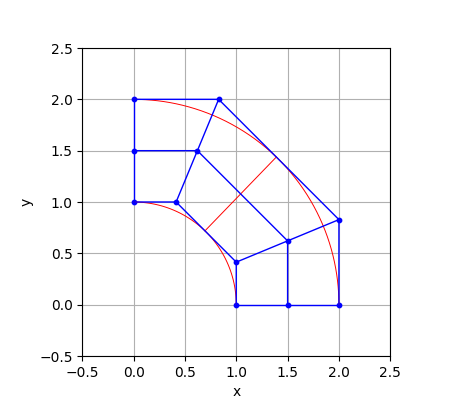
\includegraphics[keepaspectratio, scale = 1.0]
  {fig/png/09.png}
  \caption{NURBS surface and control points}
  \label{fig:nurbs surface}
\end{figure}

\newpage

\begin{figure}[htbp]
  \centering
  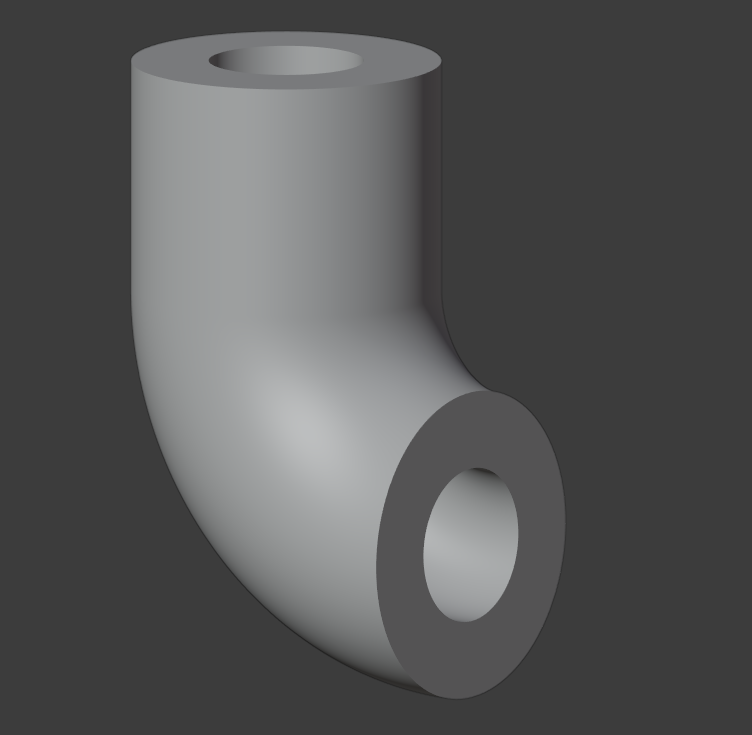
\includegraphics[keepaspectratio, scale = 0.37]
  {fig/png/04.png}
  \caption{An example of NURBS representation of a curved tube}
  \label{fig:tube}
\end{figure}

\subsection{細分化操作}
ノットベクトルとコントロールポイントを細分化する手法として,ノットインサーション(Knot Insertion)がある.
基底関数の操作は必要ないが,ノットベクトルが挿入され,コントロールポイントが増加し,さらにその物理座標が変わるため,
ノットインサーションの操作後に基底関数の計算を行う必要がある.
また,BスプラインとNURBSでやや操作が異なるため,注意が必要である.

\subsubsection{Bスプライン細分化操作}
まず,ノットベクトル$\boldsymbol{\Xi} = \{\xi_0, \xi_1, \dots, \xi_{n+p}\}$に$m$個のノットを挿入し,
挿入後のノットベクトル$\overline{\boldsymbol{\Xi}} = \{\overline{\xi}_0, \overline{\xi}_1, \dots, \overline{\xi}_{n+m+p}\}$,
コントロールポイントの行列$\boldsymbol{A} = \{\boldsymbol{B}_0, \boldsymbol{B}_1, \dots, \boldsymbol{B}_{n-1}\}^T$とすると,
ノット挿入後のコントロールポイントの行列
$\overline{\boldsymbol{A}} = \{\overline{\boldsymbol{B}}_0, \overline{\boldsymbol{B}}_1, \dots, \overline{\boldsymbol{B}}_{n+m-1}\}^T$
は以下のように表される.

\begin{equation}
  \overline{\boldsymbol{A}} = \boldsymbol{T}^p\boldsymbol{A}
  \label{eq:KI}
\end{equation}

\noindent
ここで,$\boldsymbol{T}^p$は$p = 0$のとき

\begin{equation}
  T^0_{i,j} = \left \{
  \begin{array}{l}
    1    \ \qquad $if$\  \xi_{j} \leq \overline{\xi}_i < \xi_{j + 1} \\
    0    \ \qquad $otherwise$
  \end{array}
  \right.
  \label{eq:T_0}
\end{equation}

\noindent
$p = 1,2,3,\dots$のとき

\begin{equation}
  T^p_{i,j} = \frac{\overline{\xi}_{i+p-1} - \xi_j}{\xi_{j+p-1} - \xi_j}T^{p-1}_{i,j} 
  + \frac{\xi_{j+p} - \overline{\xi}_{i+p-1}}{\xi_{j+p} - \xi_{j + 1}}T^{p-1}_{i,j+1}
  \label{eq:T_1}
\end{equation}

\noindent
以上の操作から得られたノット挿入後のノットベクトル$\overline{\boldsymbol{\Xi}}$,コントロールポイントの行列$\overline{\boldsymbol{A}}$
を用いて基底関数の計算を行うことで細分化することができる.

\subsubsection{NURBS細分化操作}
NURBSのノットインサーションでは,Bスプラインの$n$個のコントロールポイントに重みの成分を加えた行列を考え,
二次元では$\boldsymbol{B}_i = \{x_i, y_i, w_i\}(i=0,1,\dots,n-1)$をコントロールポイント座標として考える.
Bスプラインでのノットインサーションと同様に式~(\ref{eq:T_0})と式~(\ref{eq:T_1})から$\boldsymbol{T}^p$を求めた後,
式~(\ref{eq:KI})の操作を行う前に$\boldsymbol{B}_i = \{x_i\times w_i, y_i\times w_i, w_i\}(i=0,1,\dots,n-1)$と置き換えて
$\overline{\boldsymbol{A}}$を求め,さらにその成分である$\overline{\boldsymbol{B}}_j\{x_j, y_j, w_j\}(j=0,1,\dots,n+m-1)$
に対して$\overline{\boldsymbol{B}}_j\{\frac{x_j}{w_j}, \frac{y_j}{w_j}, w_j\}(j=0,1,\dots,n+m-1)$と置き換える操作を
行った後の$\overline{\boldsymbol{A}}$が細分化操作後のコントロールポイントと重みの行列となる.

NURBSのノットインサーションを行った例を図~\ref{fig:KI}に示す.

\begin{figure}[htbp]
  \centering
  \includegraphics[keepaspectratio, scale = 0.8]
  {fig/KI.ai}
  \caption{An example of NURBS Knot Insertion}
  \label{fig:KI}
\end{figure}

\subsection{高次化操作}
基底関数の次数を上げることは,式~(\ref{eq:basis func 0})と式~(\ref{eq:basis func 1})より容易であるが,
単純に次数を上げるとコントロールポイントと基底関数の線形結合で表される曲線の形状が,
次数を上げる前の曲線から変化してしまう.
形状を変えずに次数を上げ,ノットベクトルとコントロールポイントを適切に設定する高次化手法として,
オーダーエレベーション(Order Elevation)がある.
ノットインサーションと同様に基底関数を計算する前のノットベクトルとコントロールポイントに対する操作であるため,
基底関数を計算する必要はないが,非常に複雑な手順を踏む必要がある.
さらに,ノットインサーションと同様にNURBSではBスプラインと同様の操作に加えて,重みに関する処理を行う必要がある.

\subsubsection{ノット除去操作}
まず,オーダーエレベーションで必要となるノット除去操作を示す.
基本的にはノットインサーションの逆の手順を辿ることで求めることができるが,
正則ではない行列の疑似逆行列を求める過程がある.
Bスプラインのノット除去操作について考えると,
除去前のノットベクトル$\overline{\boldsymbol{\Xi}} = \{\overline{\xi}_0, \overline{\xi}_1, \dots, \overline{\xi}_{n+m+p}\}$
から$m$個のノットを除去したノットベクトル$\boldsymbol{\Xi} = \{\xi_0, \xi_1, \dots, \xi_{n+p}\}$,
ノット除去前のコントロールポイントの行列
$\overline{\boldsymbol{A}} = \{\overline{\boldsymbol{B}}_0, \overline{\boldsymbol{B}}_1, \dots, \overline{\boldsymbol{B}}_{n+m-1}\}^T$,
ノット除去後のコントロールポイントの行列$\boldsymbol{A} = \{\boldsymbol{B}_0, \boldsymbol{B}_1, \dots, \boldsymbol{B}_{n-1}\}^T$とすると,
求めたい$\boldsymbol{A}$は式~(\ref{eq:KI})と同じ式で求めることができ,$\boldsymbol{T}^p$は式~(\ref{eq:T_0})と式~(\ref{eq:T_1})から求めることができる.
$\boldsymbol{T}^p$の疑似逆行列${\boldsymbol{T}^p}^{+}$とすると,以下のように表される.

\begin{align}
  \boldsymbol{A} &= {\boldsymbol{T}^p}^{+} \overline{\boldsymbol{A}}\\
  {\boldsymbol{T}^p}^{+} &= ({\boldsymbol{T}^p}^T \boldsymbol{T}^p)^{-1} {\boldsymbol{T}^p}^T
\end{align}

\noindent
この操作を行うことで,曲線の形状を変化させることなくノットベクトルから任意のノットを取り除いたノットベクトルとコントロールポイントが得られる.

\subsubsection{Bスプライン高次化操作}
Bスプラインにおけるオーダーエレベーションの基本的な手順を以下に示す.

次数$p$とすると,
$\rm(\hspace{.18em}i\hspace{.18em})$まず,ノットベクトルの端点以外の値を重複度が$p$となるまでノットインサーションする.
ノットインサーションではBスプライン曲線形状は変化しないため,この操作により,ノットベクトルの端点以外の値で連続性が$C^0$連続となり,
Bスプライン曲線を最小のベジェ曲線(Bézier Curve)に分割することができる.
ここでベジェ曲線とは,$p+1$個のコントロールポイントから得られる$p$次曲線である.
$\rm(\hspace{.08em}ii\hspace{.08em})$次に,各ベジェ曲線で次数を上げる以下の操作を行う.
次数$p$,次数を$1$次上げた操作後の次数$\hat{p} (=p+1)$,
$p$個のコントロールポイント$\boldsymbol{B}$,操作後の$\hat{p}$個のコントロールポイント$\hat{\boldsymbol{B}}$,
$\alpha_i(i=0,1,\dots,\hat{p})$とする.

\begin{align}
  \alpha_i &= \frac{i}{\hat{p}} \\
  \hat{\boldsymbol{B}}_i &= \left \{
    \begin{array}{l}
      (1 - \alpha_i)\boldsymbol{B}_i \ \qquad \ \qquad $if$\ i = 0\\
      (1 - \alpha_i)\boldsymbol{B}_i + \alpha_i \boldsymbol{B}_{i-1} \ \ \   $otherwise$
    \end{array}
    \right.
\end{align}

\noindent
この操作を上げる次数の階数$k$だけ繰り返す.
$\rm(i\hspace{-.08em}i\hspace{-.08em}i)$その後,ノットベクトルの重複度を端点を含む全てのノットで$k$階上げる.
$\rm(i\hspace{-.08em}v\hspace{-.06em})$初めに$\rm(\hspace{.18em}i\hspace{.18em})$で挿入したノットを除去する.
以上の操作を行った後のコントロールポイントとノットベクトル,次数がそれぞれ高次化操作後の値となる.

\newpage

例として,次数$p = 2$,一様オープンノットベクトル$\boldsymbol{\Xi}=\{0,0,0,0.25,0.5,0.75,1,1,1\}$,
コントロールポイント$\boldsymbol{B} = \{(1,2),(2,1),(3,1),(3,3),(5,3),(2,5)\}^T$に対して,
次数を$1$次上げるオーダーエレベーションを行った場合の各手順での操作を以下に示す.
まず,$\rm(\hspace{.18em}i\hspace{.18em})$の操作後のBスプライン曲線を図~\ref{fig:OE_01}に示す.

\begin{figure}[htbp]
  \centering
  \includegraphics[keepaspectratio, scale = 0.8]
  {fig/OE_01.ai}
  \caption{B-Spline curve after step $\rm(\hspace{.18em}i\hspace{.18em})$ in Order Elevation}
  \label{fig:OE_01}
\end{figure}

\noindent
このとき,分割された最小のベジェ曲線は,図~\ref{fig:OE_01}におけるノットインサーション後の
$p+1$個のコントロールポイントで構成される各区間であり,それぞれのベジェ曲線に対して$\rm(\hspace{.08em}ii\hspace{.08em})$を行う.
$\rm(\hspace{.08em}ii\hspace{.08em})$及び$\rm(i\hspace{-.08em}i\hspace{-.08em}i)$の操作後のBスプライン曲線を図~\ref{fig:OE_02}に示す.

\begin{figure}[htbp]
  \centering
  \includegraphics[keepaspectratio, scale = 0.75]
  {fig/OE_02.ai}
  \caption{B-Spline curve after step $\rm(\hspace{.08em}ii\hspace{.08em})$ and $\rm(i\hspace{-.08em}i\hspace{-.08em}i)$ in Order Elevation}
  \label{fig:OE_02}
\end{figure}

\newpage

\noindent
$\rm(i\hspace{-.08em}v\hspace{-.06em})$の操作後のBスプライン曲線を図~\ref{fig:OE_03}に示す.

\begin{figure}[htbp]
  \centering
  \includegraphics[keepaspectratio, scale = 0.75]
  {fig/OE_03.ai}
  \caption{B-Spline curve after step $\rm(i\hspace{-.08em}v\hspace{-.06em})$ in Order Elevation}
  \label{fig:OE_03}
\end{figure}

\noindent
$\rm(i\hspace{-.08em}v\hspace{-.06em})$の操作後のコントロールポイント,ノットベクトル,次数がそれぞれ高次化操作後の値となる.

\subsubsection{NURBS高次化操作}
NURBSにおけるオーダーエレベーションの基本的な手順はBスプラインと同様であるが,
コントロールポイントに重みの成分を加えた行列を考え,
二次元では$\boldsymbol{B}_i = \{x_i, y_i, w_i\}(i=0,1,\dots,n-1)$をコントロールポイント座標として考える.
細分化操作でのNURBSへの拡張と同様に,$\rm(\hspace{.18em}i\hspace{.18em})$のノットインサーション,
$\rm(\hspace{.08em}ii\hspace{.08em})$の次数上げ,$\rm(i\hspace{-.08em}v\hspace{-.06em})$のノット除去の
前後でそれぞれコントロールポイント座標を置き換える操作を追加で行う必要がある.
各操作前の$n$個のコントロールポイント$\boldsymbol{B}_i = \{x_i, y_i, w_i\}(i=0,1,\dots,n-1)$を
$\boldsymbol{B}_i = \{x_i\times w_i, y_i\times w_i, w_i\}(i=0,1,\dots,n-1)$と置き換えて計算を行い,
各操作後に$m$個のコントロールポイント$\overline{\boldsymbol{B}}_j\{x_j, y_j, w_j\}(j=0,1,\dots,m-1)$を
$\overline{\boldsymbol{B}}_j\{\frac{x_j}{w_j}, \frac{y_j}{w_j}, w_j\}(j=0,1,\dots,m-1)$と置き換えることで,
NURBSでの高次化操作後のコントロールポイント,重み,ノットベクトル,次数が得られる.

\newpage

\section{アイソジオメトリック解析}
\subsection{NURBS基底関数による離散化解析}
\subsubsection{関数の定義}
物理空間からパラメータ空間への写像
$\boldsymbol{x}\ :\ \Omega \rightarrow \hat{\Omega}$は
以下のように定義される.

\begin{equation}
  \label{eq:difinement of u}
  \boldsymbol{x}(\xi)\equiv
  \begin{Bmatrix}
    x(\xi)\\
    y(\xi)
  \end{Bmatrix}
    =\sum_{a=1}^{e_{en}}N_a(\xi)
  \begin{Bmatrix}
    x^e_a\\y^e_a
  \end{Bmatrix}
\end{equation}

\noindent
ここで$N_a(\xi)$はNURBS基底関数,
${x^e_a,\ y^a_e}$は要素$e$を構成する
$a$番目のコントロールポイント$\boldsymbol{B}_a$の成分を表す.
パラメータ空間全体で他の関数についても同様に定義することができ,
パラメータ空間上の変位$\boldsymbol{u}\ :\ \Omega \rightarrow \hat{\Omega}$は
以下のように定義される.

\begin{equation}
  \boldsymbol{u}(\xi) \equiv \sum_{a=1}^{n_{en}}N_a(\xi)\boldsymbol{d}_a
\end{equation}

\noindent
ここで$\boldsymbol{d}_a$はコントロール変数と呼ばれる.

\subsubsection{境界値問題}
NURBSで定義された領域上の微分方程式を解く例として,
図~\ref{fig:boundary problem}に示すような二次元線形弾性体の境界値問題を考える.

\begin{figure}[htbp]
  \centering
  \includegraphics[keepaspectratio, scale = 0.6]
  {fig/境界値問題.ai}
  \caption{Concept of Boundary Value Problem}
  \label{fig:boundary problem}
\end{figure}

\newpage

\noindent
領域$\Omega$の固体が,物体力$\boldsymbol{b}$を受け,
ディレクレ境界$\Gamma_D$で変位固定$\overline{\boldsymbol{u}}$,
ノイマン境界$\Gamma_N$で外力$\overline{\boldsymbol{t}}$を受け,
弾性的に微小変形する.
変位$\boldsymbol{u}$,
ひずみ$\boldsymbol{\varepsilon}$,
応力$\boldsymbol{\sigma}$を求める.
領域$\Omega$の固体は,以下に示す平衡方程式(式~(\ref{eq:bvp_01})),変位ひずみ関係式(式~(\ref{eq:bvp_02})),
構成方程式(式~(\ref{eq:bvp_03})),境界条件(式~(\ref{eq:bvp_04}),式~(\ref{eq:bvp_05}))を満足する.

\begin{align}
  \label{eq:bvp_01}
  \boldsymbol{L}^T \boldsymbol{\sigma} + \boldsymbol{b} &= \boldsymbol{0} \ \ \ \qquad \qquad \rm{in} \quad \Omega\\
  \label{eq:bvp_02}
  \boldsymbol{\varepsilon} &= \boldsymbol{L} \boldsymbol{u} \qquad \qquad \rm{in} \quad \Omega\\
  \label{eq:bvp_03}
  \boldsymbol{\sigma} &= \boldsymbol{D} \boldsymbol{\varepsilon} \qquad \qquad \rm{in} \quad \Omega\\
  \label{eq:bvp_04}
  \boldsymbol{u} &= \overline{\boldsymbol{u}} \ \ \ \qquad \qquad \rm{on} \quad \Gamma_D\\
  \label{eq:bvp_05}
  \boldsymbol{t} &= \overline{\boldsymbol{t}} = \boldsymbol{n}^T \boldsymbol{\sigma} \qquad \rm{on} \quad \Gamma_N
\end{align}

\noindent
ここで,$\boldsymbol{u}$は変位ベクトル,$\boldsymbol{\varepsilon}$はひずみベクトル,
$\boldsymbol{\sigma}$は応力ベクトル,$\boldsymbol{b}$は物体力ベクトルであり,以下のように表される.

\begin{align}
  \boldsymbol{u} &= \left\{
  \begin{array}{c}
    u_1\\
    u_2
  \end{array}
  \right\}\\
  \boldsymbol{\varepsilon} &= \left\{
  \begin{array}{c}
    \varepsilon_{11}\\
    \varepsilon_{22}\\
    \gamma_{12}
  \end{array}
  \right\}\\
  \boldsymbol{\sigma} &= \left\{
  \begin{array}{c}
    \sigma_{11}\\
    \sigma_{22}\\
    \sigma_{12}
  \end{array}
  \right\}
\end{align}

\noindent
また,$\boldsymbol{L}$は微分作用素マトリクス,
$\boldsymbol{n}$は境界$\Gamma$に対する単位法線ベクトルであり,以下のように表される.

\begin{align}
  \label{eq:L}
  \boldsymbol{L} &= \left[
  \begin{array}{ccc}
    \cfrac{\partial}{\partial x} & 0\\
    0 & \cfrac{\partial}{\partial y}\\
    \cfrac{\partial}{\partial y} & \cfrac{\partial}{\partial x}
  \end{array}
  \right]\\
  \boldsymbol{n} &= \left[
    \begin{array}{ccc}
      n_1 & 0\\
      0 & n_2\\
      n_2 & n_1
    \end{array}
  \right]
\end{align}

\newpage

\noindent
$\boldsymbol{D}$は弾性マトリクスであり,ヤング率$E$,ポアソン比$\nu$とすると
平面応力状態と平面ひずみ状態でそれぞれ以下のように表される.
\begin{align}
  \label{eq:D1}
  \boldsymbol{D} &= \frac{E}{(1+\nu)(1-\nu)} \left[
    \begin{array}{ccc}
      1 & \nu & 0 \\
      \nu & 1 & 0 \\
      0 & 0 & \frac{1-\nu}{2} 
    \end{array}
  \right] &\rm{(Plane\ stress)}\\
  \label{eq:D2}
  \boldsymbol{D}&=\frac{E}{(1+\nu)(1-2\nu)} \left[
    \begin{array}{ccc}
      1-\nu & \nu & 0 \\
      \nu & 1-\nu & 0 \\
      0 & 0 & \frac{1-2\nu}{2} 
    \end{array}
  \right] &\rm{(Plane\ strain)}
\end{align}

\noindent
これらの式は境界値問題の強形式である.
強形式には唯一の厳密解が存在するが,
一般的に強形式の厳密解を解析的に求めることはできないため,
近似解を求めるための数値手法としてガラーキン法を用いる.

\subsubsection{弱形式の定義}
まず,式~(\ref{eq:bvp_01})~式~(\ref{eq:bvp_05})を近似的に満足する弱形式を定義する.
試行関数と重み関数を定義するために,$\Omega$上の自乗可積分関数空間を定義する.
この空間$L^2(\Omega)$を以下の式のような全ての関数$\boldsymbol{u}$の集合として定義する.

\begin{equation}
  \label{L2_u2_inf}
  \int_\Omega \boldsymbol{u}^2d\Omega<+\infty
\end{equation}

ここで,$d$は空間内の次元数とし,
多重指数$\boldsymbol{\alpha}\in\mathbb{N}^d$を考える.
$\boldsymbol{\alpha}=\{\alpha_1,2,\dots,\alpha_d\}$について
$|\boldsymbol{\alpha}|=\Sigma^d_{i=1}\alpha_i$を定義する.
また,微分演算子$D^j_i=\partial^j/\partial{x^j_i}$を用いて
$D^{\boldsymbol{\alpha}}=D^{\alpha_1}D^{\alpha_2}\dots D^{\alpha_d}$を定義する.
定式化に使用される特定の式が意味を成すためには
試行解の導関数が自乗可積分であることが必要であり,
$\boldsymbol{u}\ :\ \Omega\rightarrow\mathbb{R}$を試行解とすると,
次式を満たす必要がある.

\begin{equation}
  \label{nabra_u_inf}
  \int_\Omega \boldsymbol{\nabla} \boldsymbol{u}\cdot\boldsymbol{\nabla} \boldsymbol{u}d\Omega<+\infty
\end{equation}

\noindent
このような関数はソボレフ空間$H^1(\Omega)$内にある.
ソボレフ空間は以下の式で表される.

\begin{equation}
  \label{sovolev}
  H^1(\Omega)=\{\boldsymbol{u}\ |\ D^{\boldsymbol\alpha}\boldsymbol{u}\in L^2(\Omega),\ |\boldsymbol{\alpha}\le1\}
\end{equation}

\noindent
ここで$\mathcal{S}$で表す試行解の集合を,
自乗可積分微係数を持ち,$\boldsymbol{u}|_{\Gamma_D}=\overline{\boldsymbol{u}}$を満たす全ての関数として定義する.

\begin{equation}
  \label{S_trial_sol}
  \mathcal{S}=\{\boldsymbol{u}\ |\ \boldsymbol{u}\in H^1(\Omega),\ \boldsymbol{u}|_{\Gamma_D}=\overline{\boldsymbol{u}}\}
\end{equation}

\noindent
重み関数$\mathcal{V}$は以下の式で定義される.

\begin{equation}
  \label{V_trial_sol}
  \mathcal{V}=\{\boldsymbol{w}\ |\ \boldsymbol{w}\in H^1(\Omega),\ \boldsymbol{w}|_{\Gamma_D}=\boldsymbol{0}\}
\end{equation}

\noindent
式~(\ref{eq:bvp_01})に任意の重み関数$\boldsymbol{w}\in\mathcal{V}$を乗算し,
領域$\Omega$で積分することで,式~(\ref{eq:weak01})が得られる.

\begin{align}
  \int_\Omega \boldsymbol{w}^T (\boldsymbol{L}^T\boldsymbol{\sigma} + \boldsymbol{b}) d\Omega &= \boldsymbol{0} \nonumber \\
  -\int_\Omega \boldsymbol{w}^T (\boldsymbol{L}^T\boldsymbol{\sigma}) d\Omega &= \int_\Omega \boldsymbol{w}^T \boldsymbol{b} d\Omega\nonumber \\
  \label{eq:weak01}
  -\left[\int_\Omega \boldsymbol{w}^T\boldsymbol{L}^T\boldsymbol{\sigma} d\Omega - \int_\Omega (\boldsymbol{L}\boldsymbol{w})^T \boldsymbol{\sigma} d\Omega \right] &= \int_\Omega \boldsymbol{w}^T \boldsymbol{b} d\Omega
\end{align}

\noindent
ガウスの発散定理を適用することで式~(\ref{eq:weak02})が得られる.

\begin{align}
  \int_\Omega (\boldsymbol{L}\boldsymbol{w})^T \boldsymbol{\sigma} d\Omega - \int_\Gamma \boldsymbol{w}^T\boldsymbol{n}^T\boldsymbol{\sigma} d\Gamma &= \int_\Omega \boldsymbol{w}^T \boldsymbol{b} d\Omega \nonumber \\
  \label{eq:weak02}
  \int_\Omega (\boldsymbol{L}\boldsymbol{w})^T \boldsymbol{\sigma} d\Omega &= \int_\Omega \boldsymbol{w}^T \boldsymbol{b} d\Omega + \int_\Gamma \boldsymbol{w}^T \boldsymbol{t} d\Gamma
\end{align}

\noindent
ここで,$\boldsymbol{w}|_{\Gamma_D}=\boldsymbol{0}$となるので,式~(\ref{eq:weak02})の右辺第二項は以下のように表される.

\begin{align}
  \int_\Gamma \boldsymbol{w}^T \boldsymbol{t} d\Gamma &= \int_{\Gamma_N} \boldsymbol{w}^T \boldsymbol{t} d\Gamma_N + \int_{\Gamma_D} \boldsymbol{w}^T \boldsymbol{t} d\Gamma_D \nonumber \\
  \label{eq:weak03}
  &= \int_{\Gamma_N} \boldsymbol{w}^T \boldsymbol{t} d\Gamma_N
\end{align}

\noindent
また,式~(\ref{eq:bvp_05})も同様に任意の重み関数$\boldsymbol{w}\in\mathcal{V}$を乗算し,
領域$\Gamma$で積分することで,式~(\ref{eq:weak04})が得られる.

\begin{equation}
  \label{eq:weak04}
  \int _{\Gamma_N} \boldsymbol{w}^T (\boldsymbol{t} - \overline{\boldsymbol{t}}) d\Gamma = \boldsymbol{0}
\end{equation}

\newpage

\noindent
式~(\ref{eq:weak04})を式~(\ref{eq:weak03})に取り込むことで式~(\ref{eq:weak05})が得られる.

\begin{align}
  \int_\Omega (\boldsymbol{L}\boldsymbol{w})^T \boldsymbol{\sigma} d\Omega &= \int_\Omega \boldsymbol{w}^T \boldsymbol{b} d\Omega + \int_{\Gamma_N} \boldsymbol{w}^T \boldsymbol{t} d\Gamma - \int_{\Gamma_N} \boldsymbol{w}^T (\boldsymbol{t} - \overline{\boldsymbol{t}}) d\Gamma \nonumber \\
  \label{eq:weak05}
  \int_\Omega (\boldsymbol{L}\boldsymbol{w})^T \boldsymbol{\sigma} d\Omega &= \int_\Omega \boldsymbol{w}^T \boldsymbol{b} d\Omega + \int_{\Gamma_N} \boldsymbol{w}^T \overline{\boldsymbol{t}} d\Gamma
\end{align}

\noindent
応力の対称性($\sigma_{ij} = \sigma_{ji}$)と式~(\ref{eq:bvp_02}),式~(\ref{eq:bvp_03})を考慮すると,
結果として得られる問題の弱形式は以下のようになる.

\begin{equation}
  \label{eq:weak_form}
  \int_\Omega {\boldsymbol{\varepsilon}^{w}}^{T} \boldsymbol{D}\boldsymbol{\varepsilon} d\Omega = \int_\Omega \boldsymbol{w}^T \boldsymbol{b} d\Omega + \int_{\Gamma_N} \boldsymbol{w}^T \overline{\boldsymbol{t}} d\Gamma
\end{equation}

\noindent
ここで,$\boldsymbol{\varepsilon}^{w} = \boldsymbol{L}\boldsymbol{w}$である.
$\boldsymbol{a}(\boldsymbol{w},\ \boldsymbol{u})$,$\boldsymbol{L}(\boldsymbol{w})$をそれぞれ以下のように定義する.

\begin{align}
  \boldsymbol{a}(\boldsymbol{w},\ \boldsymbol{u}) &= \int_\Omega \boldsymbol{\varepsilon}^{wT} \boldsymbol{D}\boldsymbol{\varepsilon} d\Omega\\
  \boldsymbol{L}(\boldsymbol{w}) &= \int_\Omega \boldsymbol{w}^T \boldsymbol{b} d\Omega + \int_{\Gamma_N} \boldsymbol{w}^T \overline{\boldsymbol{t}} d\Gamma
\end{align}

\noindent
従って,この弱形式は以下のように書き換えることができる.

\begin{equation}
  \label{eq:weak_Galerkin}
  \boldsymbol{a}(\boldsymbol{w},\ \boldsymbol{u})=\boldsymbol{L}(\boldsymbol{w})
\end{equation}

\noindent
$\boldsymbol{a}(\cdot,\ \cdot)$は対称性を持ち,
$\boldsymbol{a}(\boldsymbol{w},\ \boldsymbol{u})=\boldsymbol{a}(\boldsymbol{u},\ \boldsymbol{w})$となる.
また,$\boldsymbol{a}(\cdot,\ \cdot)$は双線形,
$\boldsymbol{L}(\cdot)$は線形であり,全ての定数$C_1$と$C_2$に対して以下の式が成り立つ.

\begin{align}
  \boldsymbol{a} (C_1 \boldsymbol{u} + C_2 \boldsymbol{v},\ \boldsymbol{w}) &= C_1 \boldsymbol{a} (\boldsymbol{u},\ \boldsymbol{w}) + C_2 \boldsymbol{a} (\boldsymbol{v},\ \boldsymbol{w})\\
  \boldsymbol{L} (C_1 \boldsymbol{u} + C_2 \boldsymbol{v}) &= C_1 \boldsymbol{L} (\boldsymbol{u}) + C_2 \boldsymbol{L} (\boldsymbol{v})
\end{align}

\newpage

\subsubsection{ガラーキン法}
ガラ―キン法は,それぞれ$\mathcal{S}^h$と$\mathcal{V}^h$と呼ばれる
$\mathcal{S}$と$\mathcal{V}$の部分集合である有限次元近似の組み立てから成る.

\begin{align}
  \mathcal{S}^h&\subset\mathcal{S}\\
  \mathcal{V}^h&\subset\mathcal{V}
\end{align}

\noindent
式~(\ref{eq:weak_form})より,ガラーキン法の弱形式は以下のように表される.

\begin{equation}
  \label{eq:weak_form_02}
  \int_\Omega (\boldsymbol{L}\delta\boldsymbol{u}^{h})^T \boldsymbol{D}\boldsymbol{L}\boldsymbol{u}^{h} d\Omega = \int_\Omega \delta{\boldsymbol{u}^{h}}^{T} \boldsymbol{b} d\Omega + \int_{\Gamma_N} \delta{\boldsymbol{u}^{h}}^{T} \overline{\boldsymbol{t}} d\Gamma
\end{equation}

\noindent
式~(\ref{eq:weak_form_02})を式~(\ref{eq:weak_Galerkin})の形式で表したガラーキン形式は以下のように表される.

\begin{equation}
  \label{eq:Galerkin}
  \boldsymbol{a}(\delta\boldsymbol{u}^h,\ \boldsymbol{u}^h)=\boldsymbol{L}(\delta\boldsymbol{u}^h)
\end{equation}

\subsubsection{行列方程式の定義}

ガラーキン法で用いる関数空間の有限次元から関係式を導く.
解空間は任意のNURBS関数$N_A$の
線形結合で構成される.
ここで$A=1,2,\dots,n_{np}$である.
これらの関数には次式を満たす整数$n_{eq}<n_{np}$が存在すると仮定する.

\begin{equation}
  {\boldsymbol{N}_A|}_{\Gamma_D}=\boldsymbol{0}\qquad\forall A=1,2,\dots,n_{np}
\end{equation}

\noindent
定数$\boldsymbol{c}_A,A=1,2,\dots,n_{eq}$とすると,
全ての$\delta\boldsymbol{u}^h\in\mathcal{V}^h$に対して以下の式が成り立つ.

\begin{equation}
  \label{eq:delta u_vec}
  \delta\boldsymbol{u}^h=\sum^{n_{eq}}_{A=1}\boldsymbol{N}_A \boldsymbol{c}_A
\end{equation}

\noindent
$\boldsymbol{u}^h$についても同様に,$\boldsymbol{d}_A,A=1,2,\dots,n_{eq}$とすると,以下の式が成り立つ.

\begin{equation}
  \label{eq:u_vec}
  \boldsymbol{u}^h=\sum^{n_{eq}}_{A=1}\boldsymbol{N}_A \boldsymbol{d}_A
\end{equation}

\newpage

\noindent
式~(\ref{eq:Galerkin})に式~(\ref{eq:delta u_vec})と式~(\ref{eq:u_vec})を代入すると以下の式が得られる.

\begin{align}
  \boldsymbol{a} \left(
    \sum^{n_{eq}}_{A=1}\boldsymbol{N}_A\boldsymbol{c}_A,\ \sum^{n_{eq}}_{B=1}\boldsymbol{N}_B\boldsymbol{d}_B
  \right) &=
  \boldsymbol{L} \left(
    \sum^{n_{eq}}_{A=1}\boldsymbol{N}_A\boldsymbol{c}_A
  \right) \nonumber \\
  \sum^{n_{eq}}_{A=1}\boldsymbol{c}_A \left[
    \sum^{n_{eq}}_{B=1} \boldsymbol{a} (\boldsymbol{N}_A,\ \boldsymbol{N}_B\boldsymbol{d}_B) - \boldsymbol{L} (\boldsymbol{N}_A)
  \right] &= 0 \nonumber \\
  \label{eq:u temp01}
  \sum^{n_{eq}}_{A=1}\boldsymbol{c}_A \left[
    \sum^{n_{eq}}_{B=1} \boldsymbol{a} (\boldsymbol{N}_A,\ \boldsymbol{N}_B)\boldsymbol{d}_B - \boldsymbol{L} (\boldsymbol{N}_A)
  \right] &= 0
\end{align}

\noindent
式~(\ref{eq:u temp01})は任意の$\boldsymbol{c}_A$で成立するので,以下の式が成り立つ.

\begin{equation}
  \label{eq:u temp02}
  \sum^{n_{eq}}_{B=1} \boldsymbol{a} (\boldsymbol{N}_A,\ \boldsymbol{N}_B)\boldsymbol{d}_B = \boldsymbol{L} (\boldsymbol{N}_A)
\end{equation}

\noindent
ここで,以下のように定義する.

\begin{align}
  \boldsymbol{K} &= \boldsymbol{K}_{AB} = \boldsymbol{a} (\boldsymbol{N}_A, \boldsymbol{N}_B)\\
  \boldsymbol{F} &= \boldsymbol{F}_{A} = \boldsymbol{L} (\boldsymbol{N}_A)\\
  \boldsymbol{d} &= \boldsymbol{d}_B
\end{align}

\noindent
式~(\ref{eq:u temp02})は以下のような行列方程式となる.

\begin{equation}
  \label{eq:u temp03}
  \boldsymbol{K}\boldsymbol{d} = \boldsymbol{F}
\end{equation}

\noindent
ここで,$\boldsymbol{K}$は剛性マトリクス,$\boldsymbol{d}$は変位ベクトル,$\boldsymbol{F}$は外力ベクトルである.
$\boldsymbol{d}$を求めるため,式~(\ref{eq:u temp03})より以下の式を得る.

\begin{equation}
  \boldsymbol{d} = \boldsymbol{K}^{-1}\boldsymbol{F}
\end{equation}

\newpage

\subsubsection{二次元線形弾性問題}
二次元線形弾性問題においてひずみベクトルを以下のように定義する.

\begin{equation}
  \label{eq:epsilon}
  \boldsymbol{\varepsilon}=
    \begin{Bmatrix}
      \varepsilon_{11}\\
      \varepsilon_{22}\\
      \gamma_{12}
    \end{Bmatrix}=
    \begin{Bmatrix}
      \cfrac{\partial u_1}{\partial x}\\
      \cfrac{\partial u_2}{\partial y}\\
      \cfrac{\partial u_1}{\partial y}+\cfrac{\partial u_2}{\partial x}
    \end{Bmatrix}=
    \left[
      \begin{array}{cc}
        \cfrac{\partial}{\partial x} & 0\\
        0 & \cfrac{\partial}{\partial y}\\
        \cfrac{\partial}{\partial y} & \cfrac{\partial}{\partial x}
      \end{array}
    \right]
    \begin{Bmatrix}
      u_1\\
      u_2
    \end{Bmatrix}
\end{equation}

\noindent
式~(\ref{eq:u_vec})と式~(\ref{eq:epsilon})より,離散化されたひずみベクトルは以下のように表される.

\begin{equation}
  \boldsymbol{\varepsilon} = \boldsymbol{L}(\boldsymbol{N}\boldsymbol{d})=\boldsymbol{B}\boldsymbol{d}
\end{equation}

\noindent
ここで,$\boldsymbol{L}$は式~(\ref{eq:L})に示す微分作用素,$\boldsymbol{B}$は変位ひずみマトリクスであり,以下のように表される.

\begin{equation}
  \boldsymbol{B} = \boldsymbol{L}\boldsymbol{N} = \left[
    \begin{array}{cc}
       \cfrac{\partial N}{\partial x} & 0 \\
      0 & \cfrac{\partial N}{\partial y} \\
      \cfrac{\partial N}{\partial y} & \cfrac{\partial N}{\partial x} 
    \end{array}
  \right]
\end{equation}

\noindent
また,二次元線形弾性問題の応力ひずみ関係は構成方程式により定義され,
応力ベクトルは式~(\ref{eq:D1})と式~(\ref{eq:D2})に示す弾性マトリクス$\boldsymbol{D}$を用いて以下のように定義される.

\begin{equation}
  \boldsymbol{\sigma}=\boldsymbol{D}\boldsymbol{\varepsilon}
\end{equation}

\subsection{IGAにおける要素}
FEMでは節点座標を線分で繋ぐことで任意の形状のメッシュを作成し,
メッシュ内の領域を要素と定義するが,
IGAではコントロールポイント座標ではなく,
ノットベクトルで仕切られた区間を要素と定義される.
一方向について考えると,コントロールポイント数$n$個,
次数$p$とすると,ノットベクトルの長さは$n+p+1$となり,
一様オープンノットベクトルの場合,パッチ境界であるノットベクトルの両端でそれぞれ$p+1$の重複度とするため,
この方向の要素の数は$n-p$個となる.
従って,同じコントロールポイント数でも次数が異なる場合では要素数が変化する.

\newpage

\subsection{数値積分のための写像}
IGAでは数値積分法としてガウス・ルジャンドル積分法(Gauss-Legendre Quadrature)を用いる.
積分点数$n$,数値積分の重み$w_i$,被積分関数$f(x)$とすると,
ガウス・ルジャンドル積分法は以下のように定義される.

\begin{equation}
  \int^1_{-1} f(x)dx \approx \sum^n_{i=1}w_if(x_i)
\end{equation}

\noindent
積分点数によって適切な座標$x_i$と重み$w_i$を用いて計算を行うことで,
$2n-1$次関数までの正確な積分が可能となる.
ガウス積分は$[-1,1]$の領域で行う必要があるが,IGAでは要素によってノットの領域が異なるため,
図~\ref{fig:parent space}に示すような親要素空間を定義し,この空間でガウス・ルジャンドル積分を行う.

\begin{figure}[htbp]
  \centering
  \includegraphics[keepaspectratio, scale = 0.85]
  {fig/parent_space.ai}
  \caption{Physical space, Parametric space and Parent element space}
  \label{fig:parent space}
\end{figure}

\noindent
この親要素空間からパラメータ空間のそれぞれの要素へ変換し,
パラメータ空間から物理空間へ変換する,という流れで計算を行う.
物理空間の座標を$\boldsymbol{x}$,パラメータ空間の座標を$\boldsymbol{\xi}$,親要素空間の座標を$\tilde{\boldsymbol{\xi}}$
とし,
物理座標の要素を$\Omega^e$,パラメータ空間の要素を$\hat{\Omega}^e$,親要素空間の要素を$\tilde{\Omega}^e$とする.
図~\ref{fig:parent space}に示すようなパラメータ空間の要素$\hat{\Omega}^e$を考えると,
以下のような関係が成り立つ.

\begin{align}
  \label{eq:parent01}
  \xi &= \xi_i + (\tilde{\xi} + 1) \frac{\xi_{i+1} - \xi_i}{2}\\
  \label{eq:parent02}
  \eta &= \eta_j + (\tilde{\eta} + 1) \frac{\eta_{j+1} - \eta_j}{2}
\end{align}

\noindent
従って,親要素空間の座標$(\tilde{\xi},\ \tilde{\eta})\in \tilde{\Omega}^e$から
パラメータ空間の座標$(\xi,\ \eta)\in \hat{\Omega}^e$を求められる.